\documentclass[letterpaper,twoside,onecolumn,openright,final]{memoir}
%    vs.       others...   oneside twocolumn openleft  draft showtrims
%                          twoside onecolumn openany   ms
%                                            openright final 
\input lumos_common
\begin{document}
\frontmatter

\thispagestyle{empty}
\ThisLLCornerWallPaper{1}{images/4cover}
%\strut 
\vfill
\begin{center}
{\fontfamily{ppl}\fontseries{b}\fontsize{48}{50}\selectfont
Assembling the Lumos\TM\\4-Channel DC\\SSR Controller\\\strut

\vfill
}

\end{center}

\newpage
\begin{center}
\LLimg[width=1in]{danger-generic}

%DANGER! 

\mc{RISK OF FIRE, ELECTROCUTION, SERIOUS INJURY OR DEATH!} 
\end{center}

This circuit design, including but not limited to any associated plans, schematics, designs, board layouts, documentation, 
and/or components, is \mc{EXPERIMENTAL} and for \mc{EDUCATIONAL} purposes only. It is not a finished consumer-grade product.
It is assumed that you have the necessary understanding and skill to assemble and/or use electronic circuits.

Proceed \mc{ONLY} if you know exactly what you are doing, understand the proper procedures for working with the high voltage present on the components and PC boards, and understand that you do so \mc{ENTIRELY AT YOUR OWN RISK.}

The author makes \mc{NO} representation as to suitability or fitness for any purpose whatsoever, and disclaims any and all liability or warranty to the full extent permitted by applicable law.
\index{warranty, limitation of}
\index{danger warnings}
\index{warnings}

\strut\vfill
\noindent Edition 1.0, for Lumos 4-Channel DC Controller circuit version 1.0.

\smallskip


\noindent Copyright \copyright\ 2014 by Steven L. Willoughby,
Aloha, Oregon, USA.  All Rights Reserved.  
This document is released under the terms and conditions of the 
Creative Commons ``Attribution-NoDerivs 3.0 Unported'' license.  
In summary, you are free to use, reproduce, and redistribute this 
document provided you give full attribution to its author and do not
alter it or create derivative works from it.  See
\URL{http://creativecommons.org/licenses/by\-nd\-/\-3.0/} for the full
set of licensing terms.

\begin{center}
\LLimg[width=.5in]{cc}\LLimg[width=.5in]{by}\LLimg[width=.5in]{nd}
\end{center}

\newpage
\tableofcontents
\newpage
\listoffigures
\listoftables

\mainmatter

\chapter{Introduction}
\LLstart{C}{ongratulations}{on joining} the many computer-controlled
Christmas light enthusiasts, \ix{theatrical lighting} technicians, electronics hobbyists,
\index{Christmas lights}
and home automation innovators who are experimenting with new ways to have computers
control lights and other electronic devices.

The Lumos\TM\ 4-Channel DC Controller board places four such devices under the control
of your computer.  These outputs are 
electrically isolated from the logic control circuit (although the option exists to use
a common power source if the application warrants it and that isolation is not needed).

Since these boards use \acronym{RS-485} for communication, up to sixteen Lumos
boards may be ``daisy chained'' together and controlled from 
the same PC serial port.
By plugging DC-powered Christmas lights into the Lumos controller, your PC can orchestrate
a dazzling display of lights synchronized to music.

This manual details the process of assembling a Lumos controller from a bare printed
circuit board and set of components, and also shows the various optional configurations
which may be used during construction.

\section{Intended Audience}
This is an ``advanced'' level do-it-yourself electronic circuit project.  It is not
an off-the-shelf consumer-ready product.  It is only designed for educational and experimental
use by experienced hobbyists and professionals who possess the skill to construct electronic
\marginpar{\centerline{\LLimg[height=.5in]{danger-sign}}}
circuits, to understand how they function, troubleshoot problems with them, and to use them safely.

\section{Limitation of Warranty}
\index{danger warnings}
\index{warnings}
\index{warranty, limitation of}
Since this is a do-it-yourself project, the quality of the final product, and whether it 
functions as intended, is largely a result of your own efforts in building it.  As such, we
cannot offer to troubleshoot, repair, or replace a board we did not assemble for you.  Accordingly,
\marginpar{\centerline{\LLimg[height=.5in]{danger-sign}}}
these instructions, and all accompanying plans, schematics, software, hardware, and other
project materials are provided to you ``\mc{AS-IS}'' at no cost, as a courtesy between 
\acronym{DIY} hobbyists with \mc{NO WARRANTY} of any kind expressed or implied.  If you proceed
to build and/or use this unit, you do so \mc{ENTIRELY AT YOUR OWN RISK}.

If you purchased hardware materials from us (such as a PC board or programmed controller chip),
we will---at our sole discretion---replace, repair, or refund the cost of those materials if they were defective in manufacture
as shipped to you, up to 90~days from the date they were shipped to you,
but are not liable for damage caused by your handling or assembly of the unit.
Otherwise, we make no representation of suitability or fitness for any particular purpose and disclaim
all other warranty or liability of any kind to the full extent permitted by law.

\section{How to Use this Manual}
Please begin by reviewing the safety information in Chapter~\ref{ch:safety}.  

When you are ready to begin assembling your Lumos controller, gather the required tools and materials
as explained in Chapter~\ref{ch:materials}.  

Then read carefully the \emph{entire} set of instructions in the following chapters before
beginning any actual work.  Begin assembly \emph{only} if you understand all the steps you will need
to carry out.

Once your controller is complete and ready to use, refer to the separate manual,
\emph{Using the Lumos SSR Controllers} for full instructions on how to program
and use your controller.

\section{The Name of the Game}
The name ``Lumos'' is a combination of \emph{lumen}, the Latin word for ``light,''
and the initial letters of ``Orchestration System.''  Hence, ``Light Orchestration System''
which is the most common application for which the Lumos hardware and software are used---running
computerized lighting displays.

\section{Getting Additional Help}
The \ix{product website} at \URL{www.madscience.zone/lumos} contains additional documentation,
\index{website}
pointers, hints, and tips to assist you further.  If that doesn't answer all your questions,
there is an \ix{online forum} where you may submit questions for help.


\chapter{Safety Information}\label{ch:safety}

\LLstart{B}{efore}{you begin building} your Lumos controller, please take the time to
carefully read the following \ix{safety precautions}.  Failure to follow this advice could
result in death or serious injury, damage to the Lumos controller unit, and/or damage
to the other devices plugged into the controller.
\index{danger warnings}
\index{warnings}

\section{Hazardous Materials}
While assembling this unit you may come in contact with \ix{hazardous chemicals}.  The Lumos
product contains no hazardous parts \emph{per se} but if you choose to assemble it using
lead-based solder, you may expose yourself to risk of \ix{lead poisoning}.  The main cause of lead
\marginpar{\centerline{\LLimg[height=.5in]{poison_sign}}}
poisoning due to soldering is by ingesting lead particles left on your hands or work surface.
To avoid this, keep food away from your work area, and thoroughly wash your hands and work
surfaces before handling food.

In addition, if you choose to use other chemical agents (e.g., to clean excess flux from your
soldered board), be sure to read and follow their precautions and instructions carefully.

\section{Small Part Danger}
This board contains small parts which could pose a \ix{choking hazard} to small children.
This product is not a toy and is not intended for use by children in any circumstance.
The small parts on the product can be swallowed by children under 4~years of age. Keep
\marginpar{\centerline{\LLimg[height=.5in]{danger-generic}}}
out of reach of children.

\section{Hazardous Voltage}
Exercise care when working with any electrical system, including one such as the Lumos DC
controllers (even though in theory they deal with low voltages).  The power supplies of the
loads plugged into the Lumos controller, and even the power loads being controlled, may present
\marginpar{\centerline{\LLimg[width=.5in]{danger-shock}}}
a \ix{shock hazard} if not wired and handled using standard safety protocols.  Never touch or work
with live circuits. Always disconnect the power source before working on your Lumos controller.

When working with loads outdoors, be sure all supplies are plugged into \acronym{GFIC}-protected
circuits.

\section{Physical Hazards}
While assembling the unit, always wear \acronym{ANSI}-approved \ix{eye protection} gear.  When soldering,
always be aware of---and in control of---the location of your soldering iron (it will be 300$^\circ$F--500$^\circ$F---any slight 
\marginpar{\centerline{\LLimg[height=.5in]{danger-generic}}}
mistake can be costly, painful, or dangerous)! Bits of molten metal or flux can spatter onto your
skin or in your eyes during soldering.  When cutting leads, sharp metal wires may be launched into the
air, and could hit your eyes.

\section{Electrostatic Discharge (ESD) Warning}
Many of the components used in this project are sensitive to static electricity.  Always use a proper
\acronym{ESD}-safe work environment when handling them, or these parts may be permanently damaged.  If
a part is damaged in this way, 
\marginpar{\centerline{\LLimg[height=.5in]{esd_symbol_l}}}
it is impossible to tell by looking at the part, and you won't necessarily
feel the \ix{static discharge} which caused the damage.  Never take the risk of handling sensitive components
without \acronym{ESD} protection in place.
\index{danger warnings}
\index{warnings}

These parts include all transistors, voltage regulators, diodes (D0--D11),
and integrated circuits.


\section{Circuit Loading}
Always respect the maximum voltage and current capacity of the board and your wiring.  Overloading any
\index{overloaded circuits}
\index{maximum limits}
of these may result serious injury, death, fire, and/or severe damage to any or all of the devices in use.

The four output channels combined may not exceed
\marginpar{\centerline{\LLimg[height=.5in]{danger-sign}}}
10\,A total. 
Each single output channel
may not exceed 5\,A.  These should be considered \emph{absolute maximum} tolerances.  The board was designed
to operate at sustained levels below those limits.

\chapter{Before You Begin}\label{ch:before}
\LLstart{T}{HE}{Lumos controller} board may be built in a variety of different configurations
depending on how it will be used.  In order to know how to proceed from this point, you must
first decide what varition of Lumos board you wish to build.

\section{The Common ``Base'' Relay Configuration}

All boards
will contain a microcontroller and four output relays, so our assembly instructions will begin with the step-by-step 
instructions for building this portion of the board.
In the bill of materials in Chapter~\ref{ch:materials}, this is listed as the ``base'' set of
materials all Lumos boards require.

\section{Communications Options}
You will need to decide whether to use full- or half-duplex \acronym{RS-485} communications, since the parts installed
to support either option will be different.  

With the full duplex option, there are two independent data channels.  One is used for the host PC
to send commands to the Lumos board(s).  The other is used for the Lumos board(s) to respond back to
the host PC if asked to send status information about their configuration.

The half-duplex option uses \acronym{RS-485} as indicated above, but only a single data channel is used.  Most of the time,
the host PC keeps control of the wire and sends a stream of commands to the Lumos board(s) connected
to the wire.  However, if it asks one of them for a response, it must relinquish control of the line
and allow the Lumos board to assert control, transmit its response, then release control again.

With half-duplex operation, the PC needs to be able to control whether it asserts or releases control
of the serial data line.  The Lumos software assumes this is accomplished by switching the \acronym{DTR} 
line on when the PC is to transmit, and switching it off to release control and allow another device to
transmit.

Normally, we'd recommend full-duplex unless your specific needs dictate otherwise.

\section{The Sensor-In Option}
Sensor inputs \index{sensors} may be added to a Lumos board to allow for external
sensors to trigger pre-programmed relay actions.  The host PC may also monitor the
sensors.

{\bfseries At the present time, pre-programmed actions are not 
yet implemented.  The host PC
may query the Lumos board to see the status of its sensors, then command the board to do
something in response.}

A Lumos board may accommodate up to four such sensor inputs.  These are \acronym{TTL}-level inputs
which may be active low or high (although the Lumos board provides 10\,K pull-up resistors on the
sensor input lines).  These inputs take the place of the four diagnostic \acronym{LED} indicators,
so if this route is taken those will no longer be available to assist with using the board.

\chapter{What You Will Need}\label{ch:materials}
\LLstart{A}{SSEMBLING}{this project} requires soldering over 50 components onto a PC board.
Before beginning construction, be sure you have the following tools and materials on hand:
\begin{itemize}
	\item A Lumos 4-Channel DC Controller \ix{PC board}. 
		These instructions are intended for version
		1.0 of this board, which includes boards numbrered ``1.0'' and ``1.0.$x$'' where $x$ is any
		number.  If your board has a different version number printed on it, you need an
		instruction manual which was written for that board type.  \mc{DO NOT} proceed to
		use these instructions for that board!
		\index{PC board!versions}
	\item All the electronic \ix{components} required for the board.  These are listed in the
		following table.
	\item A \ix{soldering iron} with thin ``pencil'' tip.
	\item Rosin-core \ix{solder}.  
	\item Diagonal \ix{wire cutters}.
	\item \mc{ESD} protection gear such as an anti-static \ix{grounding strap}.
	\item IC \ix{chip insertion tools}.
	\item Needle-nose \ix{pliers}.
	\item A heat sink which can be clipped onto component leads while soldering.
	\item A few ounces of thermal (heat sink) grease.
\end{itemize}

\section{Bill of Materials}
Referring back to the set of options you selected in Chapter~\ref{ch:before}, add up the quantity of
parts needed for each option in the bill of materials in Table~\ref{tbl:bom}.
Note that the board is designed for miniature-size resistors and capacitors.  See the
ordering information in Chapter~\ref{ch:ordering} (p.~\pageref{ch:ordering}) for example part numbers of
components known to work with this board.

\begin{table}
\centerfloat
\begin{tabular}[c]{r|r|r|r|ll}
\toprule
\multicolumn{1}{c}{\begin{sideways}{\bfseries Base}\end{sideways}}
& \multicolumn{1}{c}{\begin{sideways}{\bfseries FDX-485} \end{sideways}}
& \multicolumn{1}{c}{\begin{sideways}{\bfseries HDX-485} \end{sideways}}
& \multicolumn{1}{c}{\begin{sideways}{\bfseries Sensor-In\quad} \end{sideways}}
& \multicolumn{1}{c}{{\bfseries Number}} 
& \multicolumn{1}{c}{{\bfseries Description}} \\
\midrule
%B  F  H  SI 
2  &  &  &  & C0--1 & Capacitors, 30\,pF or 33\,pF ceramic \\
2  &  &  &  & C2--3 & Capacitors, 0.01\,$\mu$F \\
3  &  &  &  & C4,5,7 & Capacitors, 0.1\,$\mu$F \\
2  &  &  &  & C6,8   & Capacitors, 0.33\,$\mu$F \\
\midrule
2  &  &&$-x$& D0,2  & \mc{LED}s, yellow, 3\,mm* \\
2  &  &&    & D1,4  & \mc{LED}s, green, 3\,mm\\
1  &  &&$-x$& D3    & \mc{LED}, red, 3\,mm*\\
2  &  &  &  & D5,6  & Diodes, \acronym{1N4004} \\
\midrule
1  &  &  &  & F0    & Fuse, 10\,A, Littelfuse 0297010.WXNV or equiv. \\
\midrule
5  &  &  &  & HS0--4& Heat sinks, TO-220, if needed\\
\midrule
2  &  &  & 1& J0,1,8& Terminal blocks, 5-position, Altech \mc{MBE}-155 \\
1  &  &  &  & J2    & Jumper block header, 6-position \\
3  &  &  &  & J3--5 & Jumper block headers, 4-position \\
2  &  &  &  & J6,7  & Terminal blocks, 2-position, Altech \mc{MBE}-152\\
\midrule
4  &  &  &  & Q0--3 & Transistors, \acronym{MOSFET}, FQPF13N06L \\
\midrule
1  &  &  &  & R0    & Resistor, 330\,$\Omega$, \sfrac{1}{4}\,W \\
1  &  &  &  & R1    & Resistor network, 470\,$\Omega\times$5, bussed type \\
   &  &  & 1& R2    & Resistor network, 10\,K$\times$5, bussed type\\
5  &  &  &  & R3,6--9&Resistors, 10\,K, \sfrac{1}{4}\,W \\
1  &  &  &  & R4    & Resistor, 33\,K, \sfrac{1}{4}\,W \\
1  &  &  &  & R5    & Resistor network, 680\,$\Omega\times$5, bussed type \\
4  &  &  &  & R10--13&Resistors, 470\,$\Omega$, \sfrac{1}{4}\,W\\
1  &  &  &  & R14   & Resistor network, 120\,$\Omega\times$2, isolated type \\
\midrule
1  &  &  &  & U0    & \acronym{PIC18F14K50} microcontroller, Lumos programmed \\
   &  & 1&  & U1    & \acronym{SN75176} half-duplex RS-485 driver/receiver\\
   & 1&  &  & U2    & \acronym{MAX489} full-duplex RS-485 driver/receiver\\
1  &  &  &  & U3    & \acronym{K847PH} quad opto-isolator, \mc{NPN} transistor output \\
1  &  &  &  & U4    & \acronym{LM78L05} +5\,V DC regulator, 100\,mA \\
1  &  &  &  & U5    & \acronym{LM7805} +5\,V DC regulator, 1.5\,A \\
\midrule
1  &  &  &  & X0    & Crystal, 10\,MHz \\
1  &  &  &  & XF0   & Fuse holder, Littelfuse 01530008Z, for F0 \\
6  &  &  &  & XJ0--5& Jumpers, 2-pos, 0.1$''$ pitch\\
1  &  &  &  & XR14  & \mc{SIP} socket, 4-pin, for R14\\
1  &  &  &  & XU0   & \mc{DIP} socket, 20-pin, for U0\\
   &  & 1&  & XU1   & \mc{DIP} socket, 8-pin, for U1\\
   & 1&  &  & XU2   & \mc{DIP} socket, 14-pin, for U2\\
1  &  &  &  & XU3   & \mc{DIP} socket, 16-pin, for U3\\
\bottomrule
\end{tabular}
\\{\footnotesize *Some of these are omitted in order to make room for sensor input lines.}
\caption{Lumos Bill of Materials\label{tbl:bom}}
\end{table}

\chapter{Assembling the PC Board}\label{ch:assembly}
\LLstart{W}{ITH}{all the parts} and tools at hand as described in the previous chapter, you
are now ready to begin assembly of the Lumos controller PC board.  The order of installation
presented here is intended to make assembly as convenient as possible.  Generally this means
progressing from the shortest to the tallest components, allowing the board to be laid flat
face-down on the work surface while soldering the component leads.

\begin{itemize}
\item[\HandRight] \bfseries{Note:} 
Take care to make good, solid \ix{solder connections} when installing components.
Hold your soldering iron to the part's lead \emph{and} the \ix{annular ring} of the \acronym{PCB}
until both are hot, then apply just enough solder to cover the ring, withdraw the solder, then 
remove the heat.  Good solder connections should be shiny and smooth.

\item[\HandRight] \bfseries{Note:} 
The board layout is quite compact, with many components in a small space.  Take
care when soldering that you don't accidentally heat the wrong component or form solder bridges between
nearby contact points.

\item[\HandRight] \bfseries{Note:} 
We will point out a few places where \acronym{ESD} protection is needed, but
that is intended to call attention to the issue at some key points, not to be a comprehensive list of
\emph{every} case where it is needed.  You are expected to use appropriate handling protocols for all
parts, which includes the use of \acronym{ESD} protection when working with semiconductors (e.g., all
chips, voltage regulators, transistors, etc.).
\end{itemize}

Refer to Figure~\ref{fig:placement}
throughout these instructions to see where the components are 
located on the \acronym{PCB}.  The locations are also labeled on the \acronym{PCB} itself.

\begin{figure}
\centerline{\LLimg{4SSR-DC-front}}
\caption{Lumos Board Parts Placement Diagram\label{fig:placement}}
\end{figure}
\begin{figure}
\centerline{\LLimg{4SSR-DC-back}}
\caption{Lumos Board Parts Placement (Reverse Side)\label{fig:placement-back}}
\end{figure}

\begin{enumerate}

\item\label{s:resistor1}
	Install a 330\,$\Omega$ \ix{resistor} in position R0 as marked on the \acronym{PCB}
	and Figure~\ref{fig:placement}.  This is marked with the color bands ``orange-orange-brown.'' 
	Push it all the way until flush with the \acronym{PCB}.
\item	solder the resistor leads on the bottom side of the board.  
\item\label{s:resistor2}
	Trim the excess leads with \ix{diagonal cutters}.
\item	Repeat steps \ref{s:resistor1}--\ref{s:resistor2} to 
	install (5) 10\,K \ix{resistors} (``brown-black-orange'') at R3
	and R6--R9.
\item	Repeat steps \ref{s:resistor1}--\ref{s:resistor2}
	to install (4) 470\,$\Omega$ \ix{resistors} (``yellow-violet-brown'') at R10--R13.
\item	Continue in the same way to install and solder the remaining discrete
resistor, 33\,K at position R4.
\item	{\bfseries If you will \emph{not} be installing sensor inputs,} you will not
	install the 10\,K resistor network at R2.  However, you will instead install a single
	10\,K resistor between pins 1 and 2 of R2.  See Figure~\ref{fig:r2-single} for a photo
	of what this looks like.
\begin{figure}
	\centerline{\LLimg[height=3in]{r2-single}}
	\caption{Discrete R2 Resistor If No Sensor Inputs Are Used\label{fig:r2-single}}
\end{figure}
\item	In the same fashion, install and solder (2) 30\,pF or 33\,pF \ix{capacitors} into positions marked C0--C1.
\item	Install and solder (2) 0.01\,$\mu$F capacitors into positions 
	C2--C3.
\item	Install and solder (3) 0.1\,$\mu$F capacitors into positions C4, 
	C5, and C7.
\item	Install and solder (2) 0.33\,$\mu$F capacitors into positions 
	C6 and C8.
\item	Install (2) 1N4004 \ix{diodes} at D5 and D6.  
	{\bfseries Note: These parts will not function
	if inserted the wrong direction.} Each diode has
	a stripe on one end. This end is inserted into the hole marked by the straight line (cathode)
	drawn on the \acronym{PCB}.  The unmarked end goes into the hole marked by the triangle
	(anode).  Solder into place. 
\item	Install (2) green \acronym{LED}s at D1 and D4.  
	{\bfseries Note: These must be inserted in the 
	correct orientation.} The longer lead (anode) goes into the 
	square hole, while the shorter
	lead (cathode) goes into the round hole.  Solder into place.
\item	Install (2) yellow \acronym{LED}s at D0 and D2, noting the 
	cautions from the previous step.
	{\bfseries Note: if you will be using sensor inputs, you may
	wish to omit D0 and/or D2.  See Chapter~\ref{ch:sensor-in} for 
	details before installing these parts.}
	Solder into place.
\item	Install a red \acronym{LED} at D3 as described in the previous
	two steps.  
	{\bfseries Note: if you will be using sensor inputs, you may
	wish to omit D3.  See Chapter~\ref{ch:sensor-in} for 
	details before installing this part.}
	Solder into place.
\item	Install a 20-pin \acronym{DIP} socket XU0 at position U0. Solder.
\item	Note the location of U3 and R5 (located \emph{inside} the borders 
	of chip U3).
\item	Flip the board over to the bottom (solder) side.  Be sure you still see where R5 is
	located.
\item
	Install a 680\,$\Omega$ \ix{resistor network} 
	\emph{on the bottom (solder) side} of the board at
	R5 (the row of six holes \emph{inside} U3).  {\bfseries Note the correct position of R5.} The
	square hole on the \acronym{PCB} marks where pin~1 of R5 should be inserted.  Pin~1 is marked
	with a dot on R5 itself. See Figure~\ref{fig:placement-back}.
	\marginpar{\LLimg[width=1in]{resistor-network}}
\item	Holding R5 in place, carefully flip the board over.
\item
	Keeping R5 straight, solder into place (soldering on the component side of the \acronym{PCB}).
\item	Flip the board back over to the component side.  {\bfseries Caution:} From this point 
	forward, don't forget that resistor is on the other side of the board.  If you press down
	on the board (e.g., when installing chips into sockets), you will bend R5 and may
	damage it.
\item	Install a 16-pin \acronym{DIP} socket XU3 in the position marked U3.  
	Note that it needs to fit easily
	over the soldered leads from R5.  If not, select a different style of socket or
	carefully trim down the resistor leads.
\item	Solder socket XU3.
\item	Install a 6-position \ix{jumper block} header at J2.  Solder.
\item	Install (3) 4-position \ix{jumper block} headers at J3--J5.  Solder.
\item	Install an LM78L05 voltage regulator at U4.  
	{\bfseries This part will not function unless oriented correctly.}  Note the flat side on
	the component case.  This aligns with the flat side drawn on the circuit board.
	Apply \ix{heat protection} while soldering in
	place, and/or limit soldering time to 4 seconds or less.  Use \acronym{ESD} protection.
\item	Install a \ix{fuse holders} XF0 at position F0.  Due to the wide \acronym{PCB} traces here, this may require
	extra soldering time, but be careful not to overheat the parts.
\item
	Install (2) 5-position terminal blocks at J1 and J8.  
\item
	Install (2) 2-position terminal blocks at J6 and J7.  
\item\label{s:MOSFET1}
	Using \acronym{ESD} protection, lay out (4) \acronym{MOSFET}s on your workbench.
\item	Prepare each \acronym{MOSFET} by bending the middle lead 90$^\circ$ up toward the front
	of the transistor body, then move your pliers down the lead another 0.1$''$ and bend it
	90$^\circ$
	back again, parallel to the other pins again.  It should now look like the photo
	in Figure~\ref{fig:mosfet} and should fit
	easily into the holes at Q0 on the \acronym{PCB}.
\begin{figure}
	\centerline{\LLimg[height=3in]{mosfet-side} \LLimg[height=3in]{7805-board}}
	\caption{Bending the Pins of the M\mc{OSFET}s and 7805\label{fig:mosfet}}
\end{figure}
\item	If using a heat sink, apply a \emph{small} dab of \ix{heat sink} grease on the back side of the transistor and attach the heat sink.
\item	Using appropriate heat protection and/or limiting soldering time to 4 seconds or less per
	pin, install and solder transistors Q0--Q3 onto the board.
\item\label{s:MOSFET2}
	Trim the excess leads.
\item
	Follow the same process as outlined in steps~\ref{s:MOSFET1}--\ref{s:MOSFET2}
	to install voltage regulator U5 on the board.
\item
	Install resistor network R1 onto the board, noting that pin~1 (marked
	with a dot on the resistor as was the case with R5) goes into the
	square hole marked with an arrow on the board.  Solder into place.
\item	Install and solder socket XR14 at position R14.
\item	Install fuse F0 into its socket.
\item 	Install crystal X0 onto the board without allowing it to short
	against any other component leads.  It is fine if the crystal
	is not flush against the board.  Solder into place.
\item	Using \acronym{ESD} protection, install microcontroller chip U0 into its socket.  Note the location of pin~1 of the chip, marked with a small 
	arrow or triangle on the board.
\item	Using \acronym{ESD} protection, install optoisolator chip U3 into its socket.  Note the location of pin~1 of the chip, marked with a small 
	arrow or triangle on the board.
\end{enumerate}

This completes the assembly of the main portion of the Lumos board, common to all configurations.

\bigskip

\noindent{\bfseries Continue} to the following sections
to install the other options you selected.

\chapter{Assembling the Communications Options}\label{ch:comms}
\LLstart{A}{N}{Intelligent controller board} needs some way to receive commands from the outside
world.  The Lumos 4-channel \acronym{DC} controller uses \acronym{RS-485} for this functionality,
allowing for two different options for how that is configured:
full duplex and half duplex.

\bigskip

\noindent{\bfseries Skip} to the section below which describes the communication option
you have selected.  You must do exactly {\bfseries one} of these.

\section{RS-485 Full Duplex}
Perform the following steps to add {\bfseries full-duplex} \acronym{RS-485} capability:
\begin{enumerate}
\item
	Install a 14-pin \acronym{DIP} socket XU2 at position U2.  Note the position of pin~1 (indicated
        a square pad and silk-screened triangle).  If your socket also indicates pin~1, align
	it to match the \acronym{PCB}. Solder into place.
\item	Install a MAX489 driver/receiver chip into its socket at U2, noting the marked location
	of pin~1.  Press carefully down into place.
\end{enumerate}

\bigskip\noindent{\bfseries Skip} to the next chapter.

\section{RS-485 Half Duplex}
Perform the following steps to add {\bfseries half-duplex} \acronym{RS-485} capability:
\begin{enumerate}
\item	Install an 8-pin \acronym{DIP} socket XU1 at position U1.  Note the position of pin~1 (indicated
	by a square pad and silk-screened triangle).  If your socket also indicates pin~1, align
	it to match the \acronym{PCB}. Solder into place.
\item	Install an SN75176 driver/receiver chip into its socket at U1, noting the marked location
	of pin~1.  Press carefully down into place.
\end{enumerate}

\bigskip\noindent{\bfseries Skip} to the next chapter.

\chapter{Assembling the Sensor Input Option}\label{ch:sensor-in}
\LLstart{L}{UMOS}{boards support the option} of attaching up to four simple \acronym{TTL}-level
logic inputs.  The host PC can query the Lumos board to find out the current state of these
inputs.  %The Lumos board may also be programmed to react on its own to a change in the input states.

These inputs may come from sensors (e.g., light sensors or motion sensors) which produce a compatible
output signal.  They may even come from the logic outputs of another Lumos board.

The trade-off here, however, is that the signal lines used by the sensors are also used to drive
the diagnostic \acronym{LED}s.  Any given line may only be a sensor input \emph{or} an \acronym{LED}
output at any given point in time, but never both.

It is generally recommended that you decide in advance how many sensor inputs you will need, then
look at the table of diagnostic codes in \emph{Using the Lumos SSR Controllers} to determine which
specific \acronym{LED}s you're willing to live without.  Those \acronym{LED}s should then be omitted
from the construction of the board's \acronym{CPU} option, so they won't interfere with the
inputs coming in on the same pins of the microcontroller.

The correspondence of \acronym{LED}s to inputs is shown in Table~\ref{tbl:led-inputs}.
\begin{table}[htb]
 \begin{center}
  \begin{tabular}{|c|ll|}\hline
    \bfseries Sensor & \multicolumn{2}{c|}{\bfseries Diagnostic \acronym{LED}} \\\hline\hline
    {\LARGE\strut}$\overline{\hbox{A}}$ & D0  & ``Activity'' (yellow) \\\hline
    {\LARGE\strut}$\overline{\hbox{B}}$ & D3  & ``Status'' (red) \\\hline
    {\LARGE\strut}$\overline{\hbox{C}}$ & D2  & ``Status'' (yellow) \\\hline
  \end{tabular}
 \end{center}
 \caption{\label{tbl:led-inputs}Mapping of Diagnostic \acronym{LED}s to Input Sensors}
\end{table}
Note that sensor input $\overline{\hbox{D}}$ is available without the need to remove
any \acronym{LED}s from the board.

These are named as active-low inputs (i.e., ``$\overline{\hbox{A}}$'' instead of ``A'') because that
is a common model and is compatible with the Lumos logic output lines which are active-low signals.
As such, the Lumos board includes a 10\,K pull-up resistor connected to each of the input lines
so they will default high unless explicitly pulled low by the input.  It may be actively driven low
or high by the sensor.  The Lumos board may, however, be programmed to respond to the inputs as if
they were active-high or active-low.  There shouldn't therefore be a need to invert an active-high
input for use with a Lumos board.
%\begin{figure}
% \centerfloat
% \LLimg{no-sensors-4DC}
% \LLimg{2-sensors-4DC}
% \caption{Board with No Sensors (above) and Two Sensors (below)\label{fig:pcbsensors}}
%\end{figure}

\newcommand\SensorConnectorID{J0}
\newcommand\LEDresistorValue{470}
\section{What If I Want to Keep All My LEDs?}
A natural question to ask here is, ``Can I keep the \acronym{LED}s installed \emph{and} 
have sensor inputs, deciding at different times to configure the Lumos board to treat them
as inputs or \acronym{LED}s as needed at that moment?''

The answer is ``maybe.''  It depends on what you plug into the sensor inputs and how much
current it can supply, since it would have to power the \acronym{LED}s too.  

Normally, the sensor inputs have the effective circuit shown in Figure~\ref{fig:input-normal}.
However, if the \acronym{LED} is physically present on the board at the same time, the effective
circuit becomes the one shown in Figure~\ref{fig:input-led}.  Consider whether your input source
can tolerate that circuit configuration before proceeding.  If it can't, you need to remove the
\acronym{LED}(s) corresponding to the input lines you'll use.
\begin{figure}[htb]
  \begin{circuitikz}
    \node [left] at (0,0) {Sensor Input};
    \draw (0,0) -- (1,0) -- (.8,.2) -- (1,0) -- (.8,-.2);
    \draw (1,.2) -- (1.2,0) -- (1,-.2);
    \draw (1.2,0) -- (6,0);
    \draw [thick] (8,3) -- (6,3) -- (6,-1) -- (8,-1);
    \node [right] at (6,2) {Microcontroller};
    \node [right] at (6,0) {I/O port};
    \node [below] at (1,-.2) {\SensorConnectorID};
    \draw (2,1) to [R, l={10\,K}] (2,3);
    \draw (2,1) -- (2,0);
    \draw (1.6,3) -- (2.4,3);
    \node [above] at (2,3) {+5\,V};
    \draw [fill] (2,0) circle (.1);
  \end{circuitikz}
  \caption{\label{fig:input-normal}Sensor Input Circuit}
\end{figure}
\begin{figure}[htb]
  \begin{circuitikz}
    \node [left] at (0,0) {Sensor Input};
    \draw (0,0) -- (1,0) -- (.8,.2) -- (1,0) -- (.8,-.2);
    \draw (1,.2) -- (1.2,0) -- (1,-.2);
    \draw (1.2,0) -- (6,0);
    \draw [thick] (8,3) -- (6,3) -- (6,-1) -- (8,-1);
    \node [right] at (6,2) {Microcontroller};
    \node [right] at (6,0) {I/O port};
    \node [below] at (1,-.2) {\SensorConnectorID};
    \draw (2,1) to [R, l={10\,K}] (2,3);
    \draw (2,1) -- (2,0);
    \draw (1.6,3) -- (2.4,3);
    \node [above] at (2,3) {+5\,V};
    \draw [fill] (2,0) circle (.1);
    \draw [fill] (3,0) circle (.1);
    \draw (3,0) to [full led] (3,-2);
    \draw (3,-2) to [R, l={\LEDresistorValue\,$\Omega$}] (3,-4) node[ground] {};
  \end{circuitikz}
  \caption{\label{fig:input-led}Sensor Input Circuit with \acronym{LED} Present}
\end{figure}


\newpage
\section{Installing the Option Hardware}

To install this option, do the following:
\begin{enumerate}
\item	Install a 10\,K$\times$5 resistor network at R2.  {\bfseries This component will not
	function if not oriented correctly.} Pin~1 (the common pin) is marked with a dot on the 
	resistor itself.  This goes into the hole marked with a square pad and silk-screened 
	triangle.  
	Keep the pins straight and solder R2 into place.
\item	Install a five-position terminal strip at J0.  Solder.
\end{enumerate}

\begin{description}
\item[\HandRight\ Note:] Before any inputs will be recognized, the Lumos board must be configured
in software to change those specific lines from \acronym{LED} outputs to logic inputs.  See
\emph{Using the Lumos SSR Controllers} for programming and configuration details.
{\bfseries Never attach sensors to the terminal block at any time the Lumos board is software-configur\-ed
to drive those lines as \acronym{LED}s.  
\item[\HandRight\ Note:] Always configure those as inputs before attaching the
sensor hardware.} Otherwise, the Lumos board will try to drive those \acronym{LED}s, which the
sensors may not tolerate well. If the sensor is also driving the line at the same time, you may
short out those input pins on the microcontroller, causing damage.
\end{description}

This completes the construction of the sensor input option.

\chapter{Using a Front Panel}\label{ch:fp}
\LLstart{Y}{ou}{may wish to install} your Lumos board
into a weather-resistant enclosure which allows access
to the circuit board to make connections and to access the jumper
blocks and \acronym{LED}s.
It may be desirable to bring the \acronym{LED}s, buttons,
and other connections to panel-mount components.

For power connections, there are a variety of panel-mount connectors which may be employed and wired
back to the terminal strips on the Lumos board.  Select those which work for your application.
Since the power connections need jumpers to select the input voltage, you may need to bring those
selectors out to a front or back panel as well.  You can easily connect a \acronym{DPDT} switch
to a 4-position connector which attaches to the jumper blocks.  The wiring arrangement for this 
is shown on page~\pageref{sec:voltagesw} in the appendices.

Similarly, network connections may be brought to the outside of the box by installing modular jacks
on the outside, wiring them back to J1.  In this case, \emph{both} input and output jacks should be wired
back to the terminal block.

If external \acronym{LED}s are needed, the easiest approach is to install a terminal strip at J0.
The terminals A--C on that terminal carry the same signals that run the on-board \acronym{LED}s.
(Unfortunately, the green status \acronym{LED} is not available in this manner.)
See the schematic in Figure~\ref{sch:fpex}
%See the table in Figure~\ref{tbl:input-leds} 
to find which terminal carries which \acronym{LED} power.
To avoid overloading the microcontroller's I/O port power capacity, it would be better to remove the
on-board \acronym{LED}s in the cluster D0--D4 if external \acronym{LED}s will be used
in this manner.  Note that the external \acronym{LED}s require appropriate current-limiting resistors
installed for them.  This is not provided at J0.

The Option and Reset buttons (not normally provided in any other way for the 4-channel board) 
can be external buttons which are wired to a 6-pin connector 
plugged in to J2.  An example front panel circuit is shown in Figure~\ref{sch:fpex}.

%%
%%       J11-5 J11-3    J16C J16B J16D J16-A
%
%        J2-5  J2-3     J0-A     J0-C  J0-B
%
%%        |     |         |   |    |    |
%%        o     o         A   G    Y    R
%%         | O   | R
%%        o     o         R
%%        |     |         |
%%  J2-2--*-----*---------*---*---_*----*
%%
%%
%
\begin{figure}
 \begin{circuitikz}
  \node [left] at (-.1,0) {J2-2};
  \draw [fill] (.5,0) circle (.1);
  \draw (0,0) -- +(-.2,.2) -- (0,0) -- +(-.2,-.2);
  \draw (.5,0) to [cspst, l={Option}, label/align=rotate] (.5,4) -- +(-.2,.2) -- +(0,0) -- +(.2,.2);
  \node [above] at (.5,4.2) {J2-5};
  \draw (1.5,0) to [cspst, l={Reset}, label/align=rotate] (1.5,4) -- +(-.2,.2) -- +(0,0) -- +(.2,.2);
  \node [above] at (1.5,4.2) {J2-3};
  \draw [fill] (1.5,0) circle (.1);
  \foreach \color/\x/\name/\t in {yellow/3/Activity/A, yellow/4.5/Status (Y)/C, red/6/Status (R)/B} {
	  \draw [color=\color] (\x,4) to [full led] (\x,2);
	  \draw (\x,0) to [R] (\x,2);
	  \draw (\x,4) to [empty led, l={\name}, label/align=rotate] (\x,2);
	  \draw (\x,4) -- ++(0,.2) -- +(-.2,-.2) -- +(0,0) -- +(.2,-.2);
	  \node [above] at (\x,4.2) {J0-\t};
  }
  \foreach \x in {3, 4.5, 6} {
	  \draw [fill] (\x,0) circle (.1);
  }
  \draw (0,0) -- (7.5,0);
 \end{circuitikz}
 \caption{\label{sch:fpex}Example of a Front Panel Circuit for a Lumos Board}
\end{figure}

\chapter{Going On From Here}\label{ch:goingon}
\LLstart{N}{OW}{that your Lumos controller} board is assembled, go on to read the manual
\emph{Installing the Lumos 4-Channel DC Controller} for help in setting up your controller
for use (including cabling and connector pinout information), and
\emph{Using the Lumos SSR Controllers} to learn how to control and program it using software.

\backmatter
\appendix
\renewcommand\thechapter{A}
\counterwithin{figure}{chapter}
\counterwithin{table}{chapter}
\chapter{Ordering Information}\label{ch:ordering}
%\section{Printed Circuit Boards}
%There is very small supply of Lumos printed circuit boards on hand at any given time (the number
%of boards may actually be zero).  Check the 
%project website for details.  Most likely more boards will occasionally be produced as part of a
%``co-op'' or group purchase.

%XXX ordering from batchpcb?

\section{Components}
The components used on the Lumos board are all commonly available from retail electronics suppliers.
As an example, Tables~\ref{tbl:mouserp2} and \ref{tbl:mouser} list the part numbers we used when building the prototypes,
ordered from Mouser (an on-line electronics retailer).  These specific parts are known to work with
the board and are the correct sizes to fit through all the holes.  Any equivalent parts from any
supplier should work as well.
\begin{table}
 \centerfloat
 \begin{tabular}{lllr@{}l}
  \toprule
  \multicolumn{1}{c}{\bfseries Lumos}
	&\multicolumn{1}{c}{\bfseries Mouser}
	&
	&\multicolumn{2}{c}{\bfseries Price*}
  \\
  \multicolumn{1}{c}{\bfseries Part \#}
	&\multicolumn{1}{c}{\bfseries Part \#}
	&\multicolumn{1}{c}{\bfseries Description}
	&\multicolumn{2}{c}{\bfseries (2012)}
  \\
  \midrule
HS0--4  & 532-507302B00		& Heat sink, \acronym{TO-220}, horizontal		&\$0	&.25	\\
  \midrule
XF0	& 576-01530008Z		& Fuse holder, Littelfuse 01530008Z or equiv.		& 2	&.45 \\
  \midrule
XJ0--5	  & 571-8815452		& Jumper, 2-pos., 0.1\,in pitch				&	&.12	\\
  \midrule
XR14      & Jameco 6100-1-4$\dagger$      & \acronym{SIP} socket, 4-pos., 0.1\,in pitch                   &       &.75    \\
\midrule
XU0       &	517-4820-3004-CP	& \acronym{IC} socket, \acronym{DIP}, 20-pin			&	&.42	\\
XU1       &	517-4808-3000-CP	& \acronym{IC} socket, \acronym{DIP},  8-pin			&	&.28	\\
XU2       &	517-4814-3004-CP	& \acronym{IC} socket, \acronym{DIP}, 14-pin			&	&.36	\\
XU3       &	517-4816-3004-CP	& \acronym{IC} socket, \acronym{DIP}, 16-pin			&	&.29	\\
\bottomrule
	\multicolumn{5}{p{5in}}{\footnotesize *This is not a price quote and we do not represent Mouser.com in any way. This is
simply the price \emph{we} found when we looked in 2012 and 2014, offered for general budgetary reference.  The prices shown
were for each unit, but may reflect quantity discounts we were given.
\par$\dagger$This part was found at Jameco, another online electronics outlet.
}\\
 \end{tabular}
 \caption{Component Ordering Information (accessories)\label{tbl:mouserp2}}
\end{table}
\begin{table}
 \centerfloat
 \begin{tabular}{lllr@{}l}
  \toprule
  \multicolumn{1}{c}{\bfseries Lumos}
	&\multicolumn{1}{c}{\bfseries Mouser}
	&
	&\multicolumn{2}{c}{\bfseries Price*}
  \\
  \multicolumn{1}{c}{\bfseries Part \#}
	&\multicolumn{1}{c}{\bfseries Part \#}
	&\multicolumn{1}{c}{\bfseries Description}
	&\multicolumn{2}{c}{\bfseries (2012)}
  \\
  \midrule
C0--1 & 80-C315C300J1G		& Capacitor, ceramic, 30\,pF, $\pm$5\%			&\$0	&.70 \\
C2--3 & 810-FK18C0G1H103J	& Capacitor, ceramic, 0.01\,$\mu$F, 50\,V, $\pm$5\%	&	&.21 \\
C4,5,7& 810-FK18X7R1H104K	& Capacitor, ceramic, 0.1\,$\mu$F, 50\,V, $\pm$10\%	&	&.10 \\
C6,8  & 810-FK14X7R1H334K	& Capacitor, ceramic, 0.33\,$\mu$F, 50\,V, $\pm$10\%	& 	&.186\\
  \midrule
D0,2  & 604-WP132XYD		& \acronym{LED}, yellow						&	&.06 \\
D1,4  & 604-WP132XGD		& \acronym{LED}, green						&	&.07 \\
D3    & 604-WP132XID		& \acronym{LED}, red						&	&.07 \\
D5,6  & 512-1N4004		& Diode, \acronym{1N4004}						&	&.079\\
  \midrule
F0    & 576-0297010.WXNV	& Fuse, 32\,V, 10\,A, fast-acting			&	&.526\\
  \midrule
J0,1,8& 845-MBE-155		& Terminal block, 5-pos., 5\,mm pitch			&       &.80 \\
J2 & 649-68001-106HLF 		& Header, 6-pos., 0.1\,in pitch				& 	&.28 \\
J3--5 & 649-68001-104HLF	& Header, 4-pos., 0.1\,in pitch				& 	&.202\\
J6,7  & 845-MBE-152		& Terminal block, 2-pos., 5\,mm pitch			&	&.35 \\
  \midrule
Q0--3& 512-FQPF13N06L		& Transistor, \acronym{MOSFET}, N-Channel, 60\,V	&	&.524\\
  \midrule
R0          & 660-CFS1/4C331J   	& Resistor, 330\,$\Omega$, \sfrac14\,W, mini, $\pm$5\%	&	&.15 \\
R1          & 652-4606X-1LF-470 	& Resistor network, 6-pin, 470\,$\Omega$, bussed	&	&.13 \\
R2          & 652-4606X-1LF-10K 	& Resistor network, 6-pin, 10\,K, bussed		&	&.13 \\
R3,6--9	    & 660-CFS1/4C103J   	& Resistor, 10K, \sfrac14\,W, mini, $\pm$5\%		&	&.05 \\
R4          & 660-CFS1/4C333J   	& Resistor, 33K, \sfrac14\,W, mini, $\pm$5\%		&	&.15 \\
R5          & 652-6406X-1LF-680		& Resistor network, 6-pin, 680\,$\Omega$, bussed	&	&.16 \\
R10--13	    & 660-CFS1/4C471J   	& Resistor, 470\,$\Omega$, \sfrac14\,W, mini, $\pm$5\%	&	&.05 \\
R14         & 652-4604X-2LF-120 	& Resistor network, 4-pin, 120\,$\Omega$, isolated	&	&.25 \\
  \midrule
U0          & 579-PIC18F14K50-I/P	& \acronym{PIC18F46K50} microcontroller				& 2	&.87 \\
U1   	    & 595-SN75176BP		& \acronym{SN75176} \acronym{RS-485} transceiver, half-duplex	&	&.88 \\
U2          & 700-MAX489EPD		& \acronym{MAX489} \acronym{RS-485} transceiver, full-duplex	& 4	&.11 \\
U3	    & 782-K847PH		& \acronym{K847PH} quad optocoupler, phototransistor output	&	&.827\\
U4	    & 512-LM78L05ACZXA		& \acronym{LM78L05} linear +5\,V regulator, 0.1\,A		&	&.216\\
U5	    & 511-L7805ABV		& \acronym{L7805} linear +5\,V regulator, 1.0\,A			&	&.46 \\
  \midrule
X0	    & 774-MP101			& Crystal, 10\,MHz, 30\,pF				&	&.60 \\
\bottomrule
	\multicolumn{5}{p{6in}}{\footnotesize *This is not a price quote and we do not represent Mouser.com in any way. This is
simply the price \emph{we} found when we looked in 2012 and 2014, offered for general budgetary reference.  The prices shown
were for each unit, but may reflect quantity discounts we were given.}\\
 \end{tabular}
 \caption{Component Ordering Information (electronics)\label{tbl:mouser}}
\end{table}


\chapter{Connector Pinouts}
\section{RS-485 Connection (terminal block J1)}
\begin{center}
	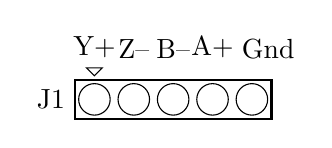
\begin{tikzpicture}[scale=.5]
		\draw [thick] (.5,.5) -- (5.5,.5) -- (5.5,1.5) -- (.5,1.5) -- cycle;
		\foreach \x in {1, 2, 3, 4, 5} {
			\draw (\x,1) circle (.4);
		}
		\node [above] at (1,1.8) {Y+};
		\node [above] at (2,1.8) {Z--};
		\node [above] at (3,1.8) {B--};
		\node [above] at (4,1.8) {A+};
		\node [above right] at (4.5,1.8) {Gnd};
		\node [left] at (.5,1) {J1};
		%\node [right] at (5.5,1) {J9};
		\draw (1,1.6) -- (0.8,1.8) -- (1.2,1.8) -- cycle;
	\end{tikzpicture}
\end{center}
Note that \acronym{RS-485} works best if the signal bus is a single line from one end to the other, with
very short ``taps'' in the line for each Lumos board.  In other words, if this is one unit in a chain, both
the input and output lines should be tied to the terminal block.  Do not ``tap in'' to the communication line and run
a single jumper out to the Lumos board.

If this is the last device in the chain, install a terminator at R14.

The main data line carrying \acronym{PC} commands to the Lumos boards connects at ``A+'' and ``B--'' (the positive
and negative signals respectively).  The return channel (for full-duplex networks) is on ``Y+'' and ``Z--''.

\section{Sensor Input Terminals (J0)}
\begin{center}
	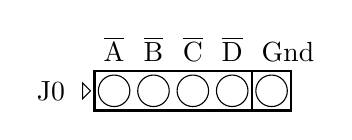
\begin{tikzpicture}[scale=.5]
		\draw [thick] (.5,.5) -- (5.5,.5) -- (5.5,1.5) -- (.5,1.5) -- cycle;
		\foreach \x in {1, 2, 3, 4, 5} {
			\draw (\x,1) circle (.4);
		}
		\draw [thick] (4.5, .5) -- (4.5, 1.5);
		\node [above] at (1,1.5) {$\overline{\hbox{A}}$};
		\node [above] at (2,1.5) {$\overline{\hbox{B}}$};
		\node [above] at (3,1.5) {$\overline{\hbox{C}}$};
		\node [above] at (4,1.5) {$\overline{\hbox{D}}$};
		\node [above right] at (4.5,1.5) {Gnd};
		\node [left] at (0,1) {J0};
		%\node [right] at (5.5,1) {J9};
		\draw (0.4,1) -- (0.2,1.2) -- (0.2,0.8) -- cycle;
	\end{tikzpicture}
\end{center}
If the Lumos controller is built to accommodate one or more sensor inputs, a set of terminals will be installed
at J0.  

It is important to note that the board's circuitry must be configured for certain inputs to be enabled
at the time the board is built, and that the board must be configured (using software) to recognize those
inputs, before they will be usable.

Each input accepts a \acronym{TTL}-level signal.  The lines are pulled up to +5\,V internally.  The board
can be configured in software to react to the inputs as active-high or active-low.

%\input dutycycle

\section{Control/ICSP Header (J2)}
\begin{center}
	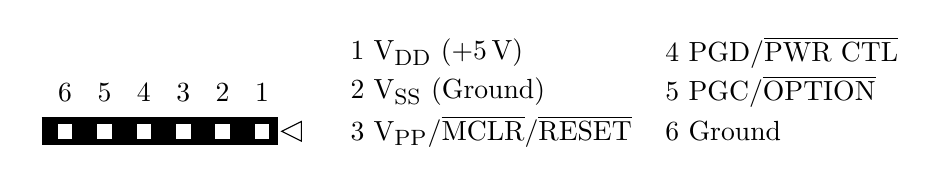
\begin{tikzpicture}[scale=.5]
		\draw [line width=10] (-.6,1)--(5.4,1);
		\foreach \x in {0, 1, 2, 3, 4, 5} {
			\foreach \y in {1} {
				\draw [fill=white] (\x-.2,\y-.2) -- (\x-.2,\y+.2) -- (\x+.2,\y+.2) -- (\x+.2,\y-.2) -- cycle;
			}
		}
		\draw (5.5,1) -- (6,1.25) -- (6,0.75) -- cycle;
		\node [above] at (0,1.5) {6};
		\node [above] at (1,1.5) {5};
		\node [above] at (2,1.5) {4};
		\node [above] at (3,1.5) {3};
		\node [above] at (4,1.5) {2};
		\node [above] at (5,1.5) {1};
		\node [right] at (7, 3.0) {1 $\hbox{V}_{\hbox{\footnotesize DD}}$ (+5\,V)};
		\node [right] at (7, 2.0) {2 $\hbox{V}_{\hbox{\footnotesize SS}}$ (Ground)};
		\node [right] at (7, 1.0) {3 $\hbox{V}_{\hbox{\footnotesize PP}}/\overline{\hbox{\mc{MCLR}}}/\overline{\hbox{\mc{RESET}}}$};
		\node [right] at (15, 3.0) {4 PGD$/\overline{\hbox{\mc{PWR CTL}}}$};
		\node [right] at (15, 2.0) {5 PGC$/\overline{\hbox{\mc{OPTION}}}$};
		\node [right] at (15, 1.0) {6 Ground};
	\end{tikzpicture}
\end{center}

This header is used for reprogramming a new firmware image onto the microcontroller chip.  Be sure to check the pinout
used by your programmer before connecting it to this port.  It may be different!

During normal operations, this header may also be used to connect off-board buttons for the reset and option functions.  
These buttons should be normally open, but connect their respective pins to ground when pushed. 
Note that the $\overline{\hbox{\mc{PWR CTL}}}$ output is only available on this header.  If the board is to be used
with a controlled power supply, a connector will need to be used to obtain this signal from J2.

\section{Voltage Select Headers (J3, J4)}\label{sec:voltagesw}
\begin{center}
	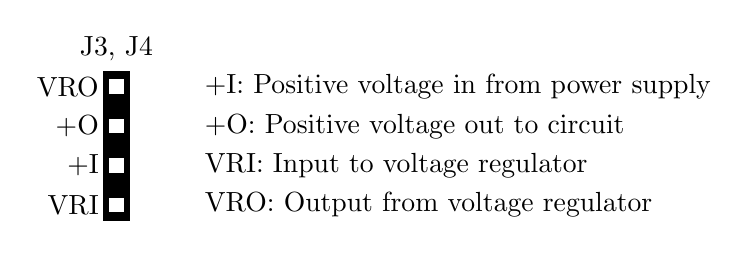
\begin{tikzpicture}[scale=.5]
		%\draw [line width=10] (.6,1)--(4.4,1);
		%\draw [line width=10] (1,.6)--(1,4.4);
		\draw [line width=10] (5,.6)--(5,4.4);
		\foreach \y in {1, 2, 3, 4} {
			\foreach \x in {5} {
				\draw [fill=white] (\x-.2,\y-.2) -- (\x-.2,\y+.2) -- (\x+.2,\y+.2) -- (\x+.2,\y-.2) -- cycle;
			}
		}
		%\node [above] at (1,4.4) {J17};
		\node [above] at (5,4.4) {J3, J4};
		%\node [left] at (.8,1) {VRO};
		%\node [left] at (.8,2) {+O};
		%\node [left] at (.8,3) {+I};
		%\node [left] at (.8,4) {VRI};
		\node [left] at (4.8,1) {VRI};
		\node [left] at (4.8,2) {+I};
		\node [left] at (4.8,3) {+O};
		\node [left] at (4.8,4) {VRO};

		\node [right] at (7, 4) {+I: Positive voltage in from power supply};
		\node [right] at (7, 3) {+O: Positive voltage out to circuit};
		\node [right] at (7, 2) {VRI: Input to voltage regulator};
		\node [right] at (7, 1) {VRO: Output from voltage regulator};
	\end{tikzpicture}
\end{center}
J3 and J4 
are used to select the input voltage supplied to the load power control and the logic portion of the board.
The square pin on the board corresponds to the VCO pin in the diagram above.
If a regulated +5\,V supply is employed, there is no
need for the on-board regulator (and in fact it can't function properly unless its input is at least +8\,V), so a jumper
is placed across the middle two pins (connecting +I and +O), bypassing the voltage regulator entirely.  \emph{In this 
case, it is critically important that the input voltage be a clean, regulated +5\,V supply.  If this voltage is exceeded,
permanent damage to the Lumos board will result!}

If +8\,V to +24\,V is attached to an input, the corresponding jumper block needs jumpers installed into the outer two pins,
connecting +I to VRI and +O to VRO.  This routes the incoming power through the voltage regulator.


\chapter{Schematics}
The following pages contain the schematic diagrams for all the various options that can comprise
a Lumos 4-channel DC controller.

\begin{figure}
\centerfloat{\LLimg[height=\textheight]{4ssr-dc-controller}}
\end{figure}
\begin{figure}
\centerfloat{\LLimg[height=\textheight]{4ssr-dc-relay}}
\end{figure}

\chapter{Glossary}\label{ch:glossary}
\begin{description}
	\item[Active High:]
		A logic signal which is considered ``on'' when the signal is ``high'' (binary 1 or +5\,V),
		and ``off'' when the signal is ``low'' (binary 0 or 0\,V).  Lumos relay circuits are 
		triggered with active-low signals.
	\item[Active Low:]
		A logic signal which is considered ``on'' and ``off'' at the opposite signal levels
		to an ``active high'' signal (q.v.).
	\item[Annular Ring:]
		The exposed ring of metal around a hole in a \acronym{PCB} where a component is to be 
		mounted.  The solder will flow across the component lead and onto the annular ring.
%	\item[Daisy Chain:]
%		The arrangement of wiring a number of devices together by connecting the first to the second,
%		then adding another connection from the second to the third, and so forth.  The network
%		connection diagram in Figure~\ref{fig:net} shows an example of a daisy chain.
	\item[\acronym{DIP} (Dual In-line Package):]
		The style of chip where the pins are laid out in two parallel rows.
	\item[\acronym{DIY}:] ``Do-It-Yourself.''
	\item[Duplex:]
		a feature of a serial line.  On a full-duplex connection, separate data wires are present
		to carry data in both directions, so one device can send and receive data at the same time.
		On a half-duplex connection, only a single set of data wires is present, so devices must
		take turns transmitting over them.
	\item[\acronym{ESD} (Electro-Static Discharge):]
		static electricity which builds on your skin and is then discharged into sensitive
		components when you touch them.  Invisible to the eye, this can punch microscopic holes
		in the inside of the components, severely damaging them.
	\item[Heat Protection:]
		A temporary heat sink applied to a component when soldering that component onto
		the \acronym{PCB}.  Typically used for heat-sens\-i\-tive components such as transistors
		and integrated circuit chips.
	\item[Jumper Block:]
		A series of pins mounted to the \acronym{PCB}.  Different options are configured for the
		circuit by placing a jumper over certain pairs of pins, shorting them together.
	\item[\acronym{LED} (Light Emitting Diode):]
		A special kind of diode which emits light when current passes from its anode to its cathode.
	\item[\acronym{MOSFET}:]
		The type of transistor which forms the major part of a Lumos DC relay channel.  The name
		is an acronym for Metal Oxide Semiconductor Field Effect Transistor.
	\item[\acronym{PCB} (Printed Circuit Board):]
		The board where electronic components are mounted to form a complete circuit.  Metal
		traces are ``printed'' (actually etched) onto the surface of the board itself to make the
		connections between components.
	\item[RS-232:]
		A standard hardware protocol for sending serial data between two devices (such as a computer
		and a modem or a single Lumos board).  Shielded cable should be used for best results, and
		the cable length should not exceed 25\,ft.
	\item[RS-485:]
		A standard hardware protocol for sending serial data between multiple devices on a single
		cable length (electrically it is a single cable which each device ``taps into'' along the
		line; physically it is typically a ``daisy chain'' arrangement where a short cable connects
		one device to the next, another cable to the next, and so on). Unshielded twisted-pair cable
		is used (like Ethernet cable), and the cable lengths should not exceed a total of 4,000\,ft
		(1,200\,m).
	\item[Terminator Plug:]
		An \acronym{RS-485} network requires a terminator at each end.  This is a small plug which plugs into
		the last unit in the daisy chain.
	\item[\acronym{TTL} (Transistor-Transistor Logic):] One of the ways digital logic circuits can be
		constructed.  For our purposes here, we consider a ``\acronym{TTL}-level'' signal to be a
		logic input or output where a voltage near +5\,V is ``high'' (binary 1 or ``true'') and a
		voltage near 0\,V is ``low'' (binary 0 or ``false'').  The inputs should never be above
		+5 nor below 0 volts.
\end{description}

\input acknowledgements

\indexintoc
\printindex
\clearpage

\input colophon

\end{document}
